\documentclass{ximera}

\usepackage{epsfig}

\graphicspath{
  {./}
  {figures/}
}


\usepackage{morewrites}

%\newcounter{ccounter}
%\setcounter{ccounter}{1}
%\newcommand{\Chapter}[1]{\setcounter{chapter}{\arabic{ccounter}}\chapter{#1}\addtocounter{ccounter}{1}}

%\newcommand{\section}[1]{\section{#1}\setcounter{thm}{0}\setcounter{equation}{0}}

%\renewcommand{\theequation}{\arabic{chapter}.\arabic{section}.\arabic{equation}}
%\renewcommand{\thefigure}{\arabic{chapter}.\arabic{figure}}
%\renewcommand{\thetable}{\arabic{chapter}.\arabic{table}}

%\newcommand{\Sec}[2]{\section{#1}\markright{\arabic{ccounter}.\arabic{section}.#2}\setcounter{equation}{0}\setcounter{thm}{0}\setcounter{figure}{0}}

\newcommand{\Sec}[2]{\section{#1}}

\setcounter{secnumdepth}{2}
%\setcounter{secnumdepth}{1} 

%\newcounter{THM}
%\renewcommand{\theTHM}{\arabic{chapter}.\arabic{section}}

\newcommand{\trademark}{{R\!\!\!\!\!\bigcirc}}
%\newtheorem{exercise}{}

\newcommand{\dfield}{{\sf dfield9}}
\newcommand{\pplane}{{\sf pplane9}}

\newcommand{\EXER}{\section*{Exercises}}%\vspace*{0.2in}\hrule\small\setcounter{exercise}{0}}
\newcommand{\CEXER}{}%\vspace{0.08in}\begin{center}Computer Exercises\end{center}}
\newcommand{\TEXER}{} %\vspace{0.08in}\begin{center}Hand Exercises\end{center}}
\newcommand{\AEXER}{} %\vspace{0.08in}\begin{center}Hand Exercises\end{center}}

% BADBAD: \newcommand{\Bbb}{\bf}

\newcommand{\R}{\mbox{$\Bbb{R}$}}
\newcommand{\C}{\mbox{$\Bbb{C}$}}
\newcommand{\Z}{\mbox{$\Bbb{Z}$}}
\newcommand{\N}{\mbox{$\Bbb{N}$}}
\newcommand{\D}{\mbox{{\bf D}}}
\usepackage{amssymb}
%\newcommand{\qed}{\hfill\mbox{\raggedright$\square$} \vspace{1ex}}
%\newcommand{\proof}{\noindent {\bf Proof:} \hspace{0.1in}}

\newcommand{\setmin}{\;\mbox{--}\;}
\newcommand{\Matlab}{{M\small{AT\-LAB}} }
\newcommand{\Matlabp}{{M\small{AT\-LAB}}}
\newcommand{\computer}{\Matlab Instructions}
\newcommand{\half}{\mbox{$\frac{1}{2}$}}
\newcommand{\compose}{\raisebox{.15ex}{\mbox{{\scriptsize$\circ$}}}}
\newcommand{\AND}{\quad\mbox{and}\quad}
\newcommand{\vect}[2]{\left(\begin{array}{c} #1_1 \\ \vdots \\
 #1_{#2}\end{array}\right)}
\newcommand{\mattwo}[4]{\left(\begin{array}{rr} #1 & #2\\ #3
&#4\end{array}\right)}
\newcommand{\mattwoc}[4]{\left(\begin{array}{cc} #1 & #2\\ #3
&#4\end{array}\right)}
\newcommand{\vectwo}[2]{\left(\begin{array}{r} #1 \\ #2\end{array}\right)}
\newcommand{\vectwoc}[2]{\left(\begin{array}{c} #1 \\ #2\end{array}\right)}



\newcommand{\inv}{^{-1}}
\newcommand{\CC}{{\cal C}}
\newcommand{\CCone}{\CC^1}
\newcommand{\Span}{{\rm span}}
\newcommand{\rank}{{\rm rank}}
\newcommand{\trace}{{\rm tr}}
\newcommand{\RE}{{\rm Re}}
\newcommand{\IM}{{\rm Im}}
\newcommand{\nulls}{{\rm null\;space}}

\newcommand{\dps}{\displaystyle}
\newcommand{\arraystart}{\renewcommand{\arraystretch}{1.8}}
\newcommand{\arrayfinish}{\renewcommand{\arraystretch}{1.2}}
\newcommand{\Start}[1]{\vspace{0.08in}\noindent {\bf Section~\ref{#1}}}
\newcommand{\exer}[1]{\noindent {\bf \ref{#1}}}
\newcommand{\ans}{}
\newcommand{\matthree}[9]{\left(\begin{array}{rrr} #1 & #2 & #3 \\ #4 & #5 & #6
\\ #7 & #8 & #9\end{array}\right)}
\newcommand{\cvectwo}[2]{\left(\begin{array}{c} #1 \\ #2\end{array}\right)}
\newcommand{\cmatthree}[9]{\left(\begin{array}{ccc} #1 & #2 & #3 \\ #4 & #5 &
#6 \\ #7 & #8 & #9\end{array}\right)}
\newcommand{\vecthree}[3]{\left(\begin{array}{r} #1 \\ #2 \\
#3\end{array}\right)}
\newcommand{\cvecthree}[3]{\left(\begin{array}{c} #1 \\ #2 \\
#3\end{array}\right)}
\newcommand{\cmattwo}[4]{\left(\begin{array}{cc} #1 & #2\\ #3
&#4\end{array}\right)}

\newcommand{\Matrix}[1]{\ensuremath{\left(\begin{array}{rrrrrrrrrrrrrrrrrr} #1 \end{array}\right)}}

\newcommand{\Matrixc}[1]{\ensuremath{\left(\begin{array}{cccccccccccc} #1 \end{array}\right)}}



\renewcommand{\labelenumi}{\theenumi)}
\newenvironment{enumeratea}%
{\begingroup
 \renewcommand{\theenumi}{\alph{enumi}}
 \renewcommand{\labelenumi}{(\theenumi)}
 \begin{enumerate}}
 {\end{enumerate}\endgroup}



\newcounter{help}
\renewcommand{\thehelp}{\thesection.\arabic{equation}}

%\newenvironment{equation*}%
%{\renewcommand\endequation{\eqno (\theequation)* $$}%
%   \begin{equation}}%
%   {\end{equation}\renewcommand\endequation{\eqno \@eqnnum
%$$\global\@ignoretrue}}

%\input{psfig.tex}

\author{Martin Golubitsky and Michael Dellnitz}

%\newenvironment{matlabEquation}%
%{\renewcommand\endequation{\eqno (\theequation*) $$}%
%   \begin{equation}}%
%   {\end{equation}\renewcommand\endequation{\eqno \@eqnnum
% $$\global\@ignoretrue}}

\newcommand{\soln}{\textbf{Solution:} }
\newcommand{\exercap}[1]{\centerline{Figure~\ref{#1}}}
\newcommand{\exercaptwo}[1]{\centerline{Figure~\ref{#1}a\hspace{2.1in}
Figure~\ref{#1}b}}
\newcommand{\exercapthree}[1]{\centerline{Figure~\ref{#1}a\hspace{1.2in}
Figure~\ref{#1}b\hspace{1.2in}Figure~\ref{#1}c}}
\newcommand{\para}{\hspace{0.4in}}

\renewenvironment{solution}{\suppress}{\endsuppress}

\ifxake
\newenvironment{matlabEquation}{\begin{equation}}{\end{equation}}
\else
\newenvironment{matlabEquation}%
{\let\oldtheequation\theequation\renewcommand{\theequation}{\oldtheequation*}\begin{equation}}%
  {\end{equation}\let\theequation\oldtheequation}
\fi

\makeatother


\title{Nonconstant Coefficient Linear Equations}

\begin{document}
\begin{abstract}
\end{abstract}
\maketitle


\label{sec:VarConstS}

The simplest nonconstant coefficient homogeneous\index{homogeneous} 
linear differential equation is:
\begin{equation}   \label{eq:linhomo1}
\frac{dx}{dt}  =  a(t)x.
\end{equation}
This equation does not have constant coefficients, since the coefficient 
$a$ depends on $t$.  The equation is linear as linear combinations of 
solutions are solutions.  Note that \Ref{eq:linhomo1} is of the form 
\Ref{eq:ghivp} and can be solved by separation of variables. 
\index{separation of variables}

If $x(t_0)=0$, then $x(t)=0$ is the solution to the initial value problem
\Ref{eq:linhomo1}.
To solve the initial value problem $x(t_0)=x_0$ for \Ref{eq:linhomo1}
when $x_0\neq 0$, we apply the technique of separation of variables to 
this equation, which yields
\[
\ln|x| = H(t) + C,
\]
where $H(t)$ is the definite integral
\begin{equation}   \label{e:H(t)}
H(t)=\int_{t_0}^t a(\tau)d\tau.
\end{equation}
Exponentiation implies that
\[
x(t) = Ke^{H(t)}
\]
for an appropriate scalar $K$.  Indeed, if $x(t_0)=x_0$, then
\[
x_0 = x(t_0) = Ke^{H(t_0)} = Ke^0 = K.
\]
We have shown that the function 
\begin{equation} \label{E:ssv}
x(t) = x_0 e^{H(t)}
\end{equation}
is the unique solution\index{uniqueness of solutions} 
to the initial value problem\index{initial value problem} 
\Ref{eq:linhomo1} where $x(t_0)=x_0$.

\subsubsection*{An Example of a Nonconstant Coefficient Equation}

We illustrate \Ref{E:ssv} by an example. Solve the initial value problem
\[
\begin{array}{rcl}
\dps \frac{dx}{dt} & = & -\dps \frac{x}{t} \\
x(2) & = & 5.
\end{array}
\]
Since $a(t)=-\frac{1}{t}$, we can use \Ref{e:H(t)} to compute
\[
H(t)=-\int_2^t \frac{1}{\tau}d\tau = -\ln t +\ln 2 =
\ln\left(\frac{2}{t}\right).
\]
Then the solution \Ref{E:ssv} is given by
\[
x(t) = 5 e^{\ln(2/t)} = \frac{10}{t}.
\]

\subsection*{The Inhomogeneous Equation}
\index{inhomogeneous}

Next, we consider forced linear differential equations of the type
\begin{equation}   \label{eq:linode1}
\frac{dx}{dt} = a(t)x + g(t),
\end{equation}
where $a$ and $g$ are continuous functions of $t$.  The differential  
equation \Ref{eq:linode1} is homogeneous when $g=0$  and 
\index{homogeneous} inhomogeneous otherwise.  As is always the 
case, we find the general solution\index{general solution} 
to the inhomogeneous equation 
by adding the general solution to the homogeneous equation (that
we can find by separation of variables) to a particular solution to 
the inhomogeneous equation.  

\subsubsection*{Two Examples of Solutions of Inhomogeneous Equations}

(a) Find all solutions of the differential equation
\begin{equation} \label{E:ie1}
\frac{dx}{dt} = 3t^2x + 3t^2.
\end{equation}
By inspection, the constant function $x_p(t)=-1$ is a 
particular solution\index{particular solution} 
of \Ref{E:ie1}. 
Since all solutions of the homogeneous equation are of the form $Ke^{t^3}$
for some real constant $K$, it follows that the general solution of the 
inhomogeneous equation is
\[
x(t) = -1 + Ke^{t^3}.
\]

\noindent (b) Find all solutions of the differential equation
\begin{equation}  \label{E:ie2}
\frac{dx}{dt} = \left(\frac{5}{t}-t\right) x + t^6.
\end{equation}
A calculation shows that $x_p(t)=t^5$ is a particular solution of \Ref{E:ie2}. 
Since all solutions to the homogeneous equation are of the form 
$Kt^5 e^{-t^2/2}$ for some real constant $K$, it follows that the general
solution of the inhomogeneous equation is
\[
x(t) = t^5 + Kt^5 e^{-t^2/2}.
\]

\subsection*{Inhomogeneous Equations and Variation of Parameters}
\index{variation of parameters}

In Examples~\Ref{E:ie1} and \Ref{E:ie2} we guessed or were given a
particular solution\index{particular solution!variation of parameters} 
to the inhomogeneous equation.  Now we discuss 
a method for finding a particular solution to the inhomogeneous
equation \Ref{eq:linode1} when $g(t)$ is a nonzero function.   This 
technique for finding a particular solution is called 
{\em variation of parameters\/}.  

We already know by separation of variables that every solution of the 
{\em homogeneous\/} equation ($g=0$) has the form $Ke^{H(t)}$ where 
$\frac{dH}{dt}=a$.  The idea behind variation of parameters is to
allow $K$ to depend on $t$.    \index{variation of parameters}
More precisely, assume that a solution $x(t)$ has the form
\[
x(t) = c(t)e^{H(t)},
\]
where $c$ is a differentiable function of $t$.  Substituting $x(t)$ in 
\Ref{eq:linode1}, using the product rule for differentiation and suppressing
the explicit dependence of functions on $t$, leads to the identity
\[
\frac{dc}{dt}e^{H}+ce^{H}a =  ace^{H}+g,
\]
which simplifies to
\[
\frac{dc}{dt} = ge^{-H}.
\]
This last equation may be solved for $c(t)$ by integration, obtaining
\begin{equation}   \label{eq:c(t)}
c(t) = \int g(\tau)e^{-H(\tau)}d\tau.
\end{equation}
Uniqueness of solutions\index{uniqueness of solutions} to initial 
value problems implies the main result of this section.

\begin{theorem}[Variation of Parameters]  \label{thm:varpar}
\index{variation of parameters}
The unique solution to the initial value problem
\index{variation of parameters!initial value problem}
\[
\begin{array}{rcl}
\dps \frac{dx}{dt} & = & a(t)x+g(t) \\
x(t_0) & = & x_0.
\end{array}
\]
is
\[
x(t) = c(t)e^{H(t)},
\]
where 
\[
H(t)=\int_{t_0}^t a(\tau)d\tau \AND
c(t)=\int_{t_0}^t g(\tau)e^{-H(\tau)}d\tau + x_0.
\]
\end{theorem} \index{variation of parameters}


\subsubsection*{Two Examples of Variation of Parameters}

(a)   Solve the initial value problem
\begin{equation} \label{e:solntheq}
\begin{array}{rcl}
\dps \frac{dx}{dt} & = & -\dps \frac{x}{t} + \frac{2}{t^4}\\
x(1) & = & 0.
\end{array}
\end{equation}
Compute
\[
H(t)= -\int_1^t\frac{1}{\tau}d\tau = -\ln t +\ln 1 = -\ln t.
\]
Hence 
\[
c(t)=\int_1^t \frac{2}{\tau^4}e^{\ln\tau}d\tau + 0
=\int_1^t \frac{2}{\tau^3} d\tau = -\frac{1}{t^2}+1
\]
which implies that 
\begin{equation}  \label{e:solnth}
x(t)=\left(1-\frac{1}{t^2}\right)\frac{1}{t}
\end{equation}
is the solution. For comparison we show the graph of \Ref{e:solnth} in 
Figure~\ref{F:solnmd}(left) and the result of a numerical computation of 
the initial value problem using {\sf dfield5}\index{\computer!dfield5} 
in Figure~\ref{F:solnmd}(right).

\begin{figure}[htb]
           \centerline{%
           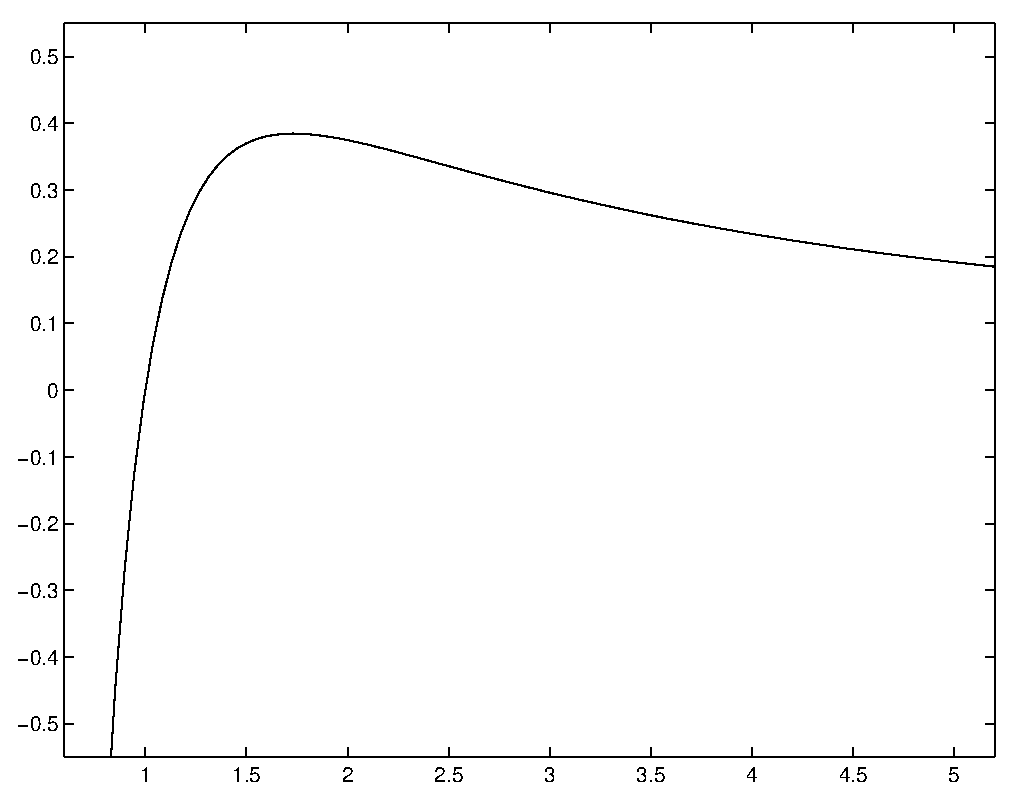
\psfig{file=../figures/solnm.eps,width=2.8in}
           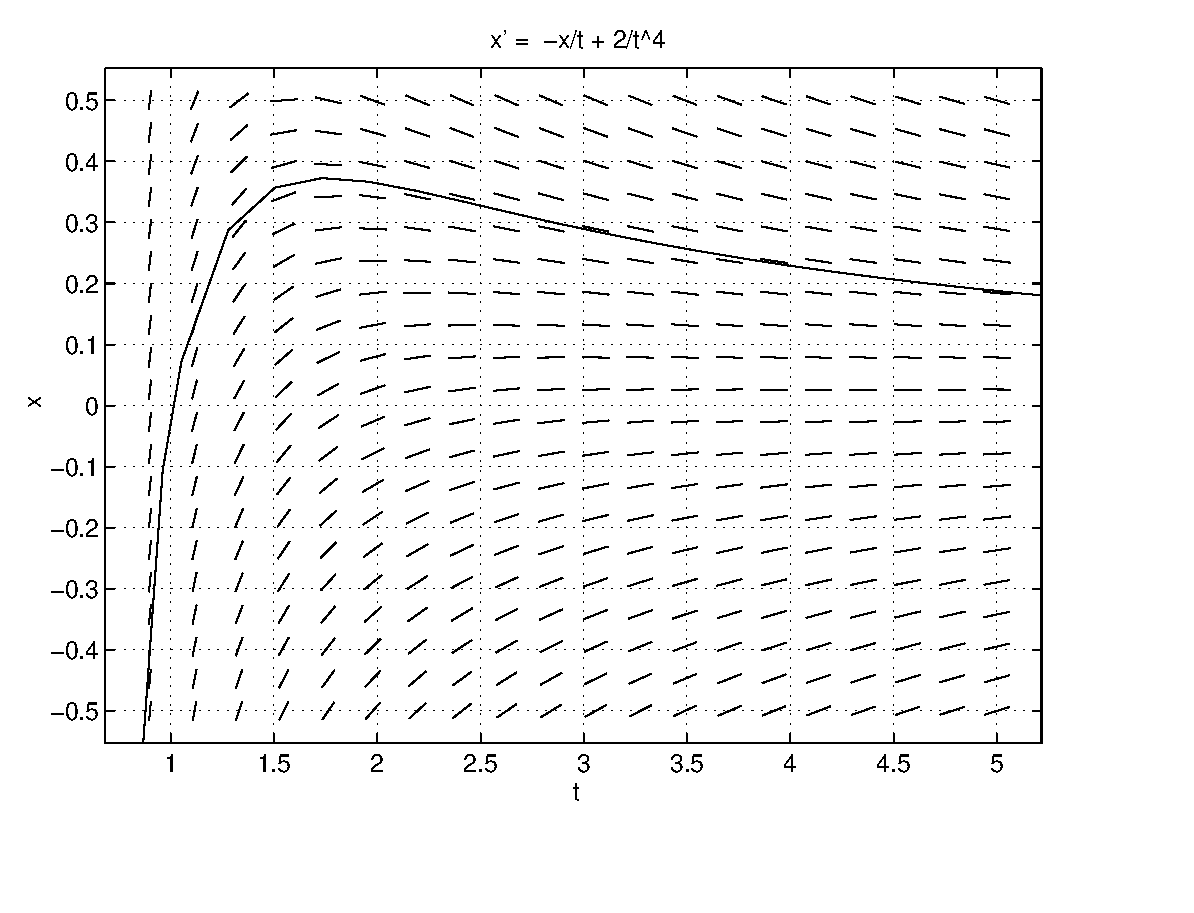
\psfig{file=../figures/solnd.eps,width=3.0in}}
           \caption{(Left) Graph of solution~\protect\Ref{e:solnth} to equation 
	\protect\Ref{e:solntheq}. (Right) The time series for solution to 
	\protect\Ref{e:solntheq} with initial condition $x(1)=0$ using 
	{\sf dfield5}.}
           \label{F:solnmd}
\end{figure}

\noindent (b) Solve the initial value problem
\[
\begin{array}{rcl}
\dps \frac{dx}{dt} & = & 4x + \cos t + e^{2t} \\
x(0) & = & 1.
\end{array}
\]
Here $H(t)=4t$ and 
\begin{eqnarray*}
c(t) & = &  \int_0^t g(\tau)e^{-4\tau} d\tau +1\\
& = & \int_0^t \left(\cos\tau + e^{2\tau}\right)e^{-4\tau} d\tau
+1\\
& = & \frac{1}{17}\left( e^{-4t}(\sin t - 4\cos t)+4\right) +
\frac{1}{2}\left(1-e^{-2t}\right) + 1.
\end{eqnarray*}
Thus, the solution is
\[
x(t)=c(t) e^{4t} = \frac{1}{17}(\sin t - 4\cos t+4e^{4t}) -
\frac{1}{2}e^{2t} + \frac{3}{2}e^{4t}.
\]


\EXER

\TEXER 

\noindent In Exercises~\ref{c14.2.1a} -- \ref{c14.2.1f} decide whether 
or not the given differential equation is linear.  If it is linear, 
specify whether the equation is homogeneous or inhomogeneous.
\begin{exercise}  \label{c14.2.1a}
$\dps \frac{dx}{dt} = 0$.
\end{exercise}
\begin{exercise}  \label{c14.2.1b}
$\dps \frac{dx}{dt} = x^2\cos t$.
\end{exercise}
\begin{exercise}  \label{c14.2.1c}
$\dps \frac{dx}{dt} = x+t^2$.
\end{exercise}
\begin{exercise}  \label{c14.2.1d}
$\dps \frac{dx}{dt} = \frac{t}{x}-\frac{1}{t}$.
\end{exercise}
\begin{exercise}  \label{c14.2.1e}
$\dps (t^2+1)\frac{dx}{dt} = x+\sin t$.
\end{exercise}
\begin{exercise} \label{c14.2.1f}
$\dps x\frac{dx}{dt} = \cos t$
\end{exercise}

\noindent In Exercises~\ref{c14.2.6a} -- \ref{c14.2.6d} solve the given 
initial value problems by variation of parameters.
\begin{exercise}   \label{c14.2.6a}
$\dps \frac{dx}{dt} = t^2 x + t^2, \quad x(1)=1$.
\end{exercise}
\begin{exercise}   \label{c14.2.6b}
$\dps \frac{dx}{dt} = x+2t, \quad x(0)=-1$.
\end{exercise}
\begin{exercise}   \label{c14.2.6c}
$\dps \frac{dx}{dt} = 
\frac{t}{t^2+1}x+\sin(t)\sqrt{t^2+1},\quad x(0)=2$.
\end{exercise}
\begin{exercise}   \label{c14.2.6d}
$\dps \frac{dx}{dt} = 2x+\frac{1}{t}e^{2t}, \quad x(1)=4$.
\end{exercise}



\CEXER

\noindent In Exercises~\ref{c14.2.11a} -- \ref{c14.2.11c} use 
{\sf dfield5}\index{\computer!dfield5} 
to compute solutions to the given linear differential equations.  What is 
the asymptotic behavior of the solutions as $t$ tends to infinity?  Use 
variation of parameters to explain the behavior.
\begin{exercise}   \label{c14.2.11a}
$\dps\frac{dx}{dt} = -2 x + t$.
\end{exercise}
\begin{exercise}   \label{c14.2.11b}
$\dps\frac{dx}{dt} = -2 x + t^2$.
\end{exercise}
\begin{exercise}   \label{c14.2.11c}
$\dps\frac{dx}{dt} = -2 x + \sin t$.
\end{exercise}




\end{document}
